        
    \subsection*{Introducing our offset}
        
        Now that we have handled the case where our linear separator is on the \textbf{origin}, we want to \textbf{shift} our separator \textbf{away} from it.
        
        In our \textbf{1-D} case, we easily \textbf{shifted} away from the origin: any separator $x_1>C$ where $C$ \textbf{isn't zero}, we shift by $C$ units.
        
        \begin{figure}[H]
            \centering
                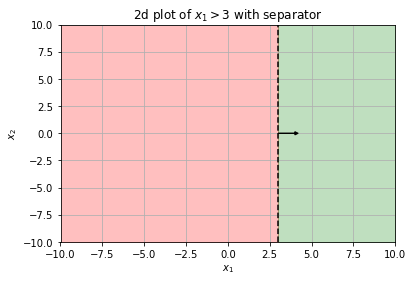
\includegraphics[width=70mm,scale=0.5]{images/classification_images/x1_2d_plot_separator.png}
                \caption*{By making our inequality $x_1>3$ \textbf{nonzero}, we moved away from the origin by 3 units!}
        \end{figure}
        
        We could make our inequality \textbf{nonzero}, then! That could move us \textbf{away} from the origin, just in a different \textbf{direction}.
        
        Or, we could equivalently do this...
            \note{Note: $A \Longleftrightarrow B$ means $A$ and $B$ are equivalent!}
        
        \begin{equation}
            x_1 >3 \Longleftrightarrow x_1-3 > 0
        \end{equation}
        
        So, instead, we could just add a constant to our expression, which we will call $\theta_0$.
        
        We'll also switch out $\theta \cdot x = \theta^T x$.\\
        
        \begin{kequation}
            A general \vocab{linear separator} can do \vocab{binary classification} using the hypothesis
            
            \begin{equation*}
                h(x; \theta) = \text{sign}(\theta^T x + \theta_0 )= 
                \begin{cases}
                    +1 & \text{if $\theta^T x + \theta_0 > 0$} \\
                    -1 & \text{otherwise}
                \end{cases}
            \end{equation*}
        \end{kequation}
        
        Notice that this looks very similar to what we did in regression! We'll get into that in a bit.
        
        First, a quick look at the components of our equation:\\
        
        \begin{concept}
            For \vocab{binary classification}, $\theta$ and $\theta_0$ entirely \purp{define} our \vocab{linear separator}.
            
            \begin{itemize}
                \item $\theta$ gives us the \purp{orientation} of our line.
                \item $\theta_0$ \purp{shifts} that line around in \gren{space}.
            \end{itemize}
        \end{concept}
    
    \subsection*{How does the offset affect our classifier?}
    
        So, how exactly does our offset $\theta_0$ affect our \textbf{classifier}? Well, we mark our classifier with our \textbf{normal vector} and the \textbf{boundary}.
        
        Our \textbf{normal vector} is entirely captured by $\theta$: it's unchanged by $\theta_0$.
        
        What about our \textbf{boundary}? We have its \textbf{orientation}, but we don't know where it has \textbf{shifted} to.
        
        \begin{figure}[H]
            \centering
                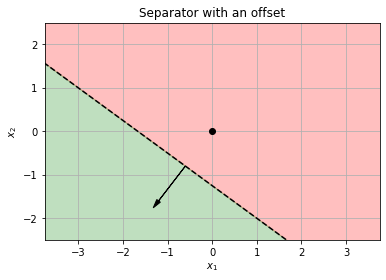
\includegraphics[width=70mm,scale=0.5]{images/classification_images/separator_with_offset.png}
                \caption*{Note that the origin has been marked.}
        \end{figure}
        
        Well, let's use our equation: the \textbf{boundary} line is given by 
        
        \begin{equation}
            \theta^T x + \theta_0 = 0 
            \Longleftrightarrow 
            \theta^T x = -\theta_0
        \end{equation}
        
        We'll break the effects of $\theta_0$ into three cases:
            \note{Note: the below statements are true no matter what $\theta$ we choose!}
        
        For each, we'll show two different $\theta$ values.
        
        \begin{itemize}
            \item If $\theta_0=0$, then $x=(0,0)$ is \textbf{on the line}.
                \begin{itemize}
                    \item Without an \textbf{offset}, our line goes through the \textbf{origin}.
                \end{itemize}
                
                \begin{figure}[H]
                    \centering                         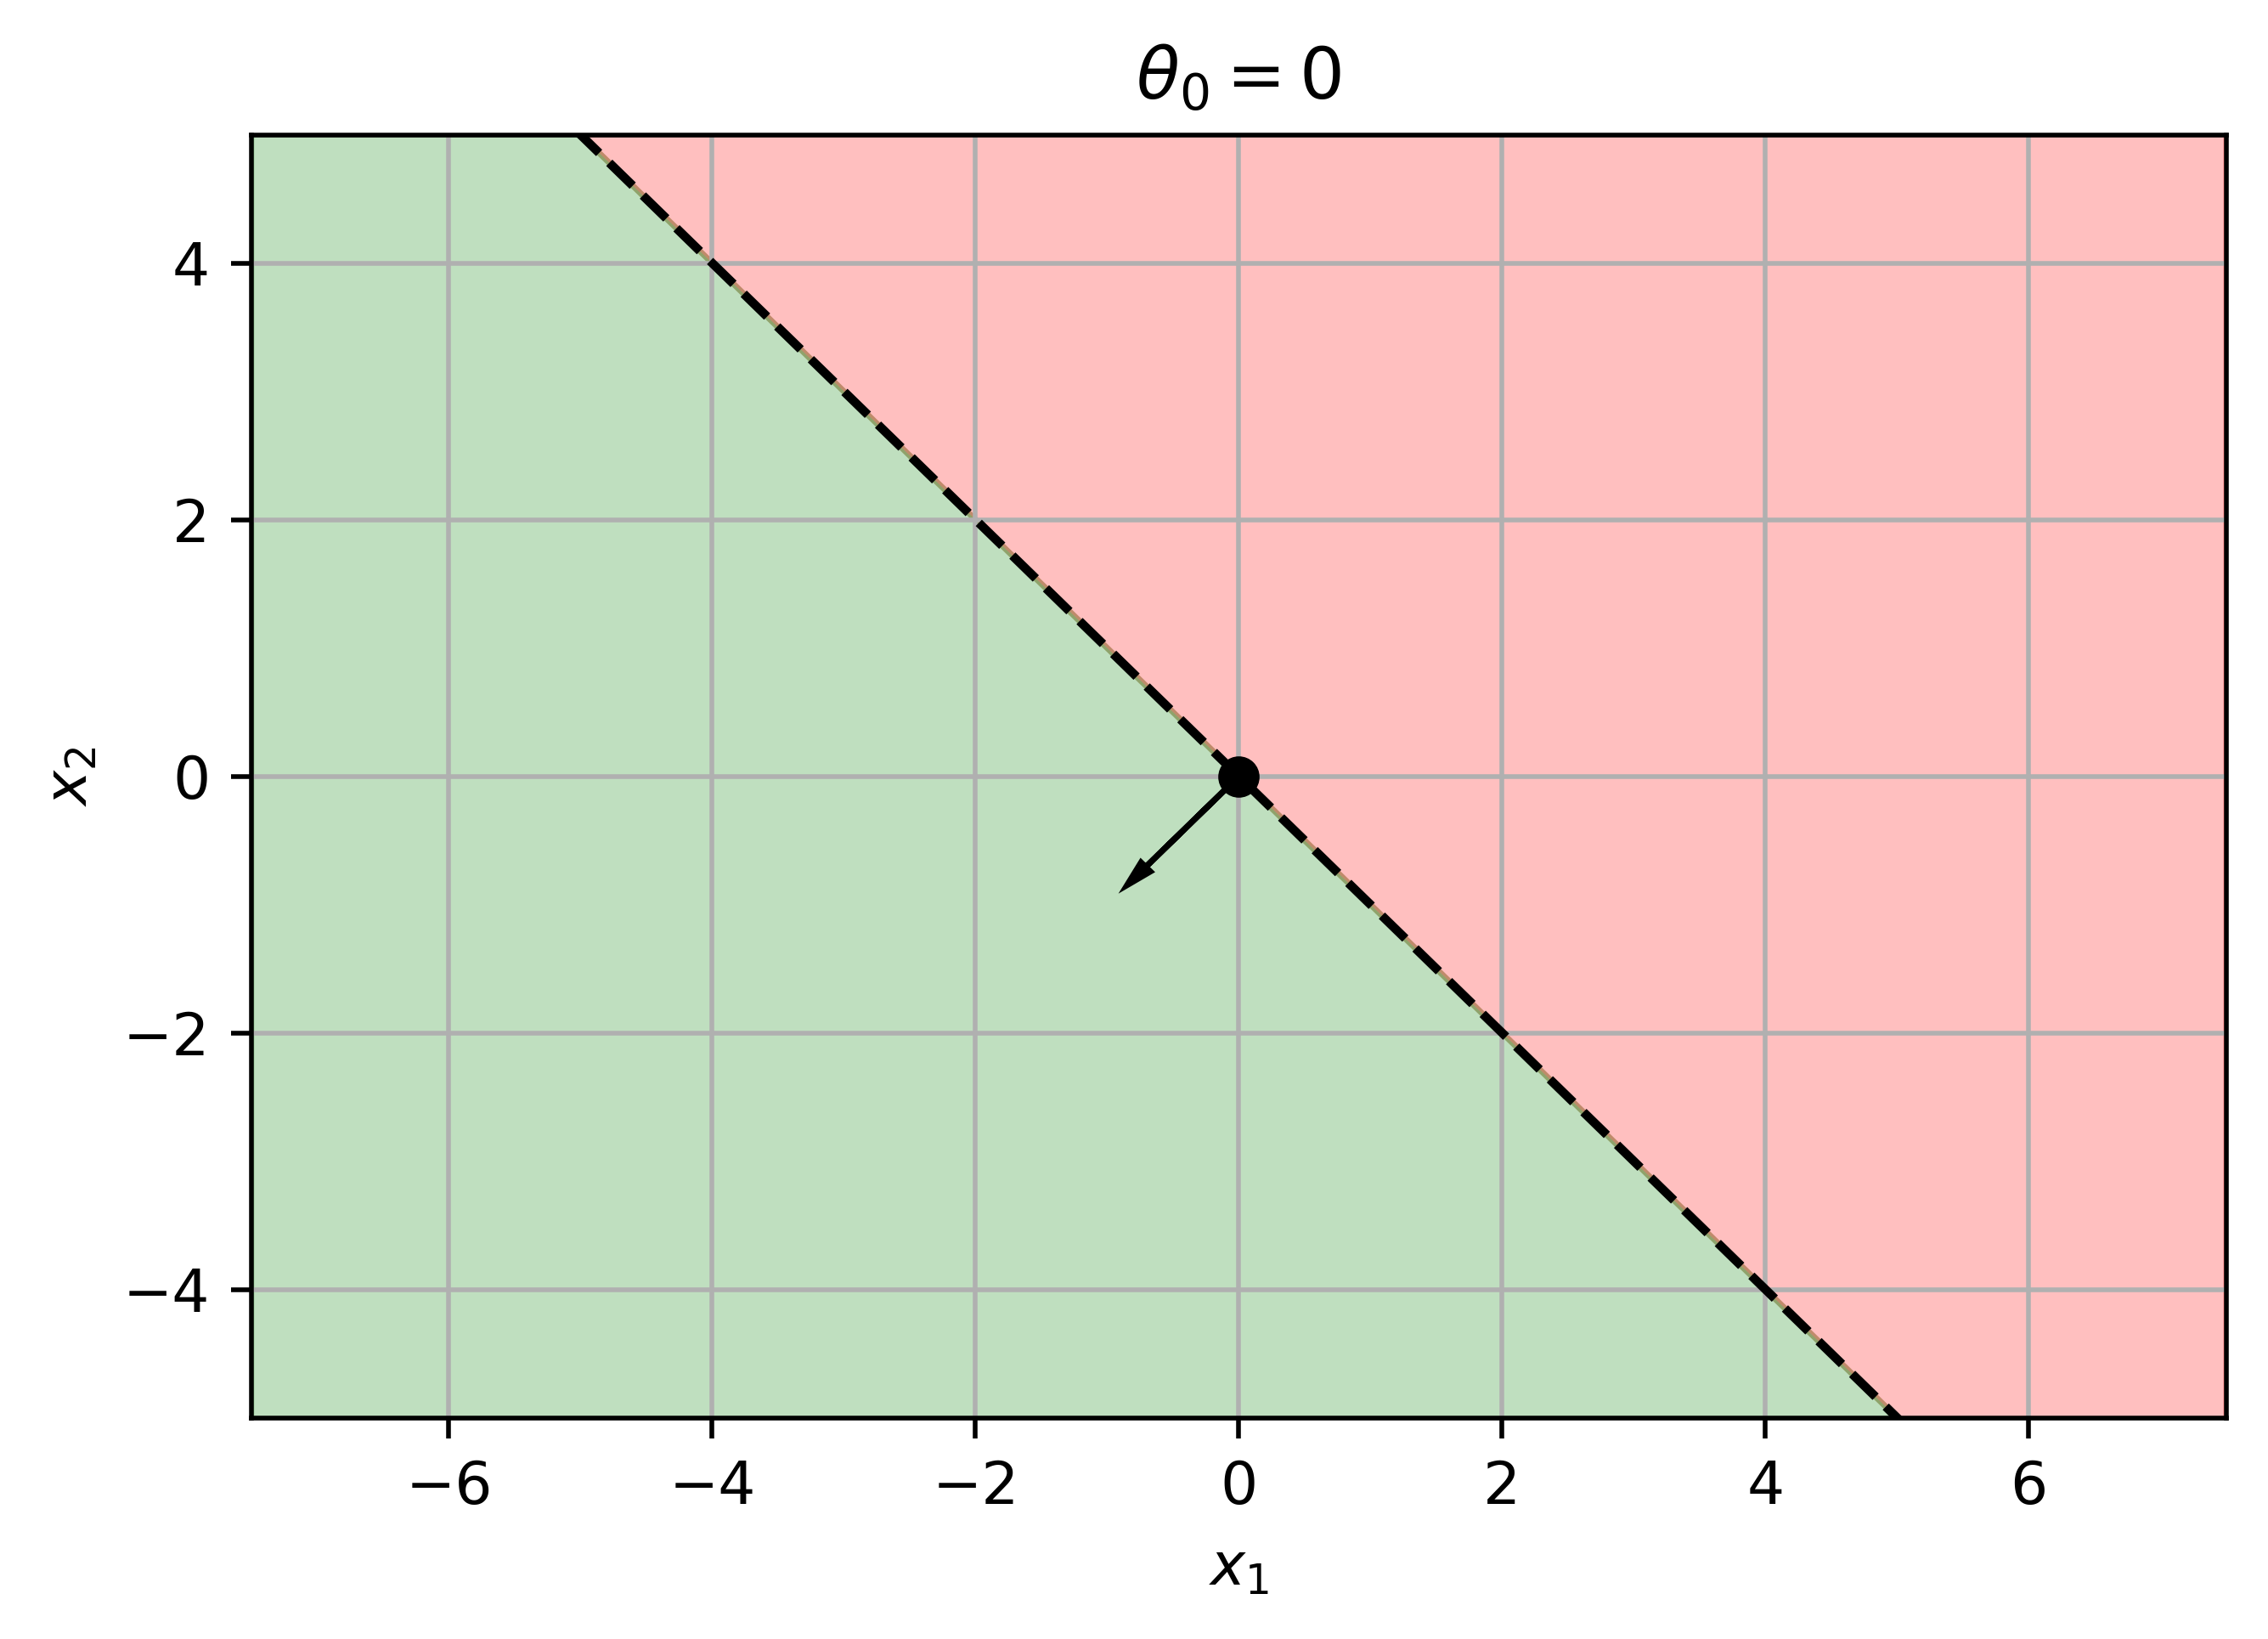
\includegraphics[width=60mm,scale=0.5]{images/classification_images/theta_0_zero.png}
                    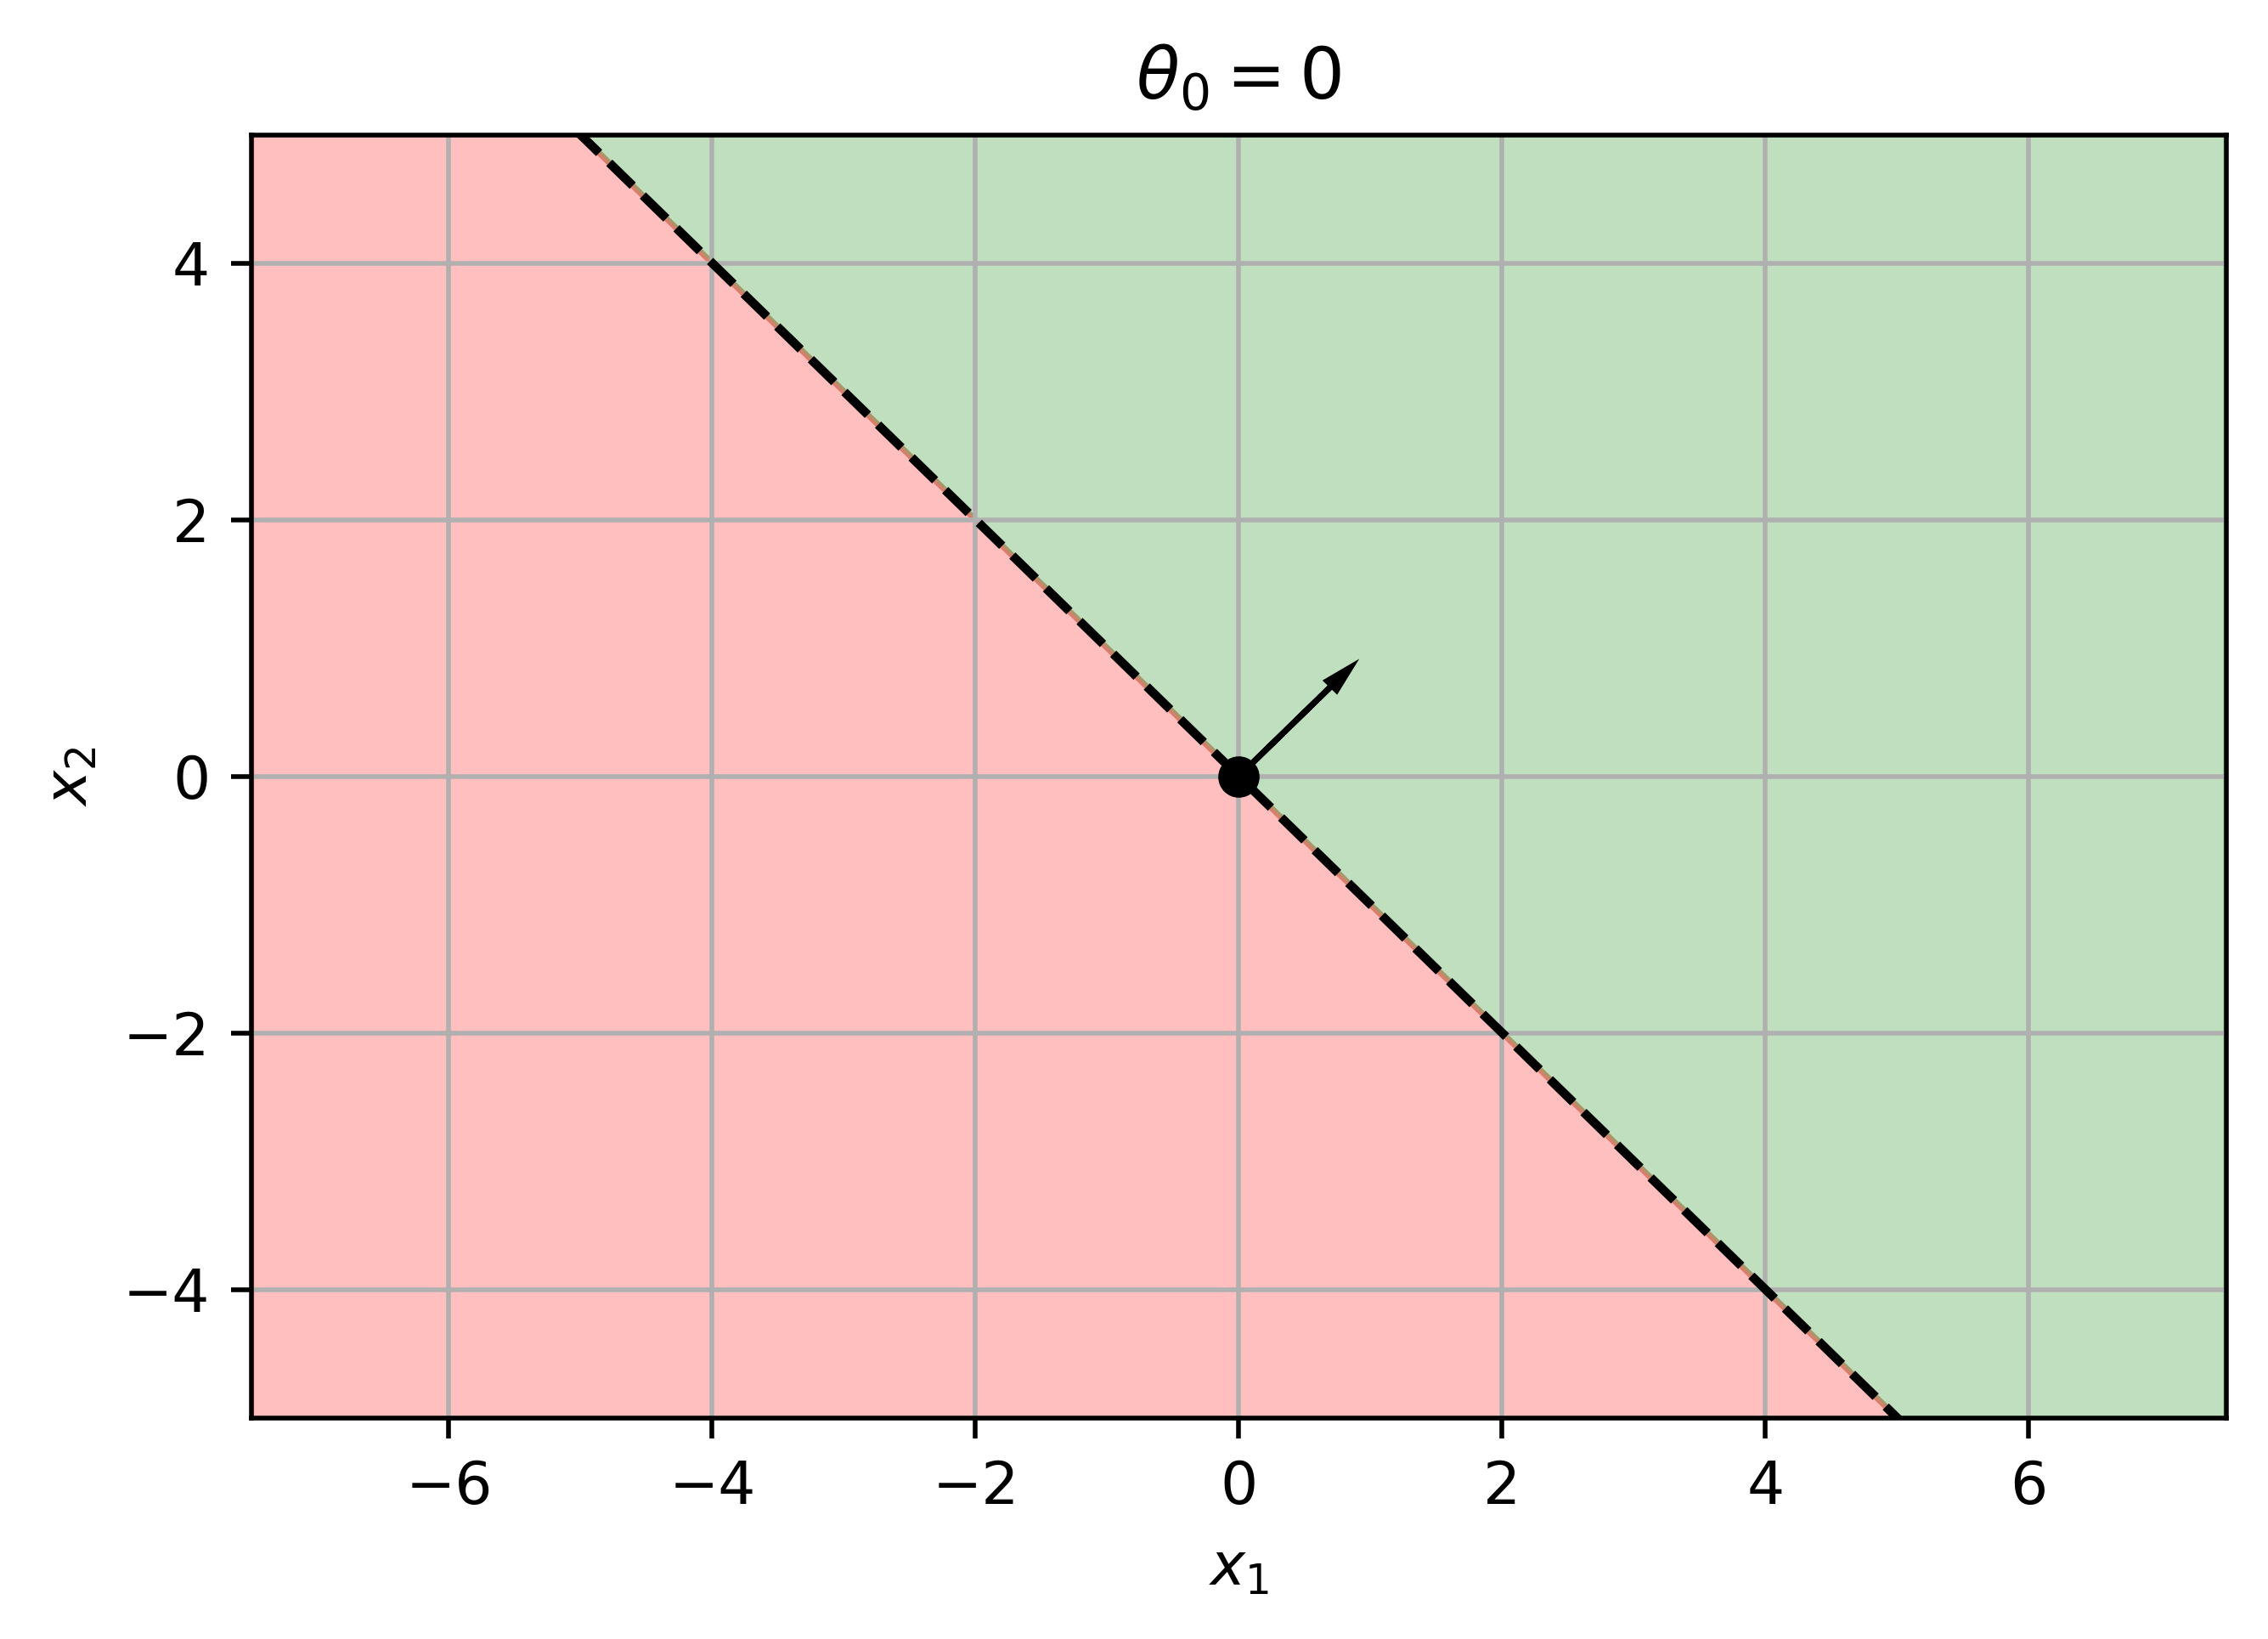
\includegraphics[width=60mm,scale=0.5]{images/classification_images/zero_theta0_positive_theta.png}
                        \caption*{The boundary is on the origin.}
                \end{figure}
                
            \item If $\theta_0>0$, then $x=(0,0)$ is in the \textbf{positive} region.
                \begin{itemize}
                    \item That means the positive region is \textbf{larger}: the line must have moved in the $-\theta$ direction.
                \end{itemize}
                
                \begin{figure}[H]
                    \centering                         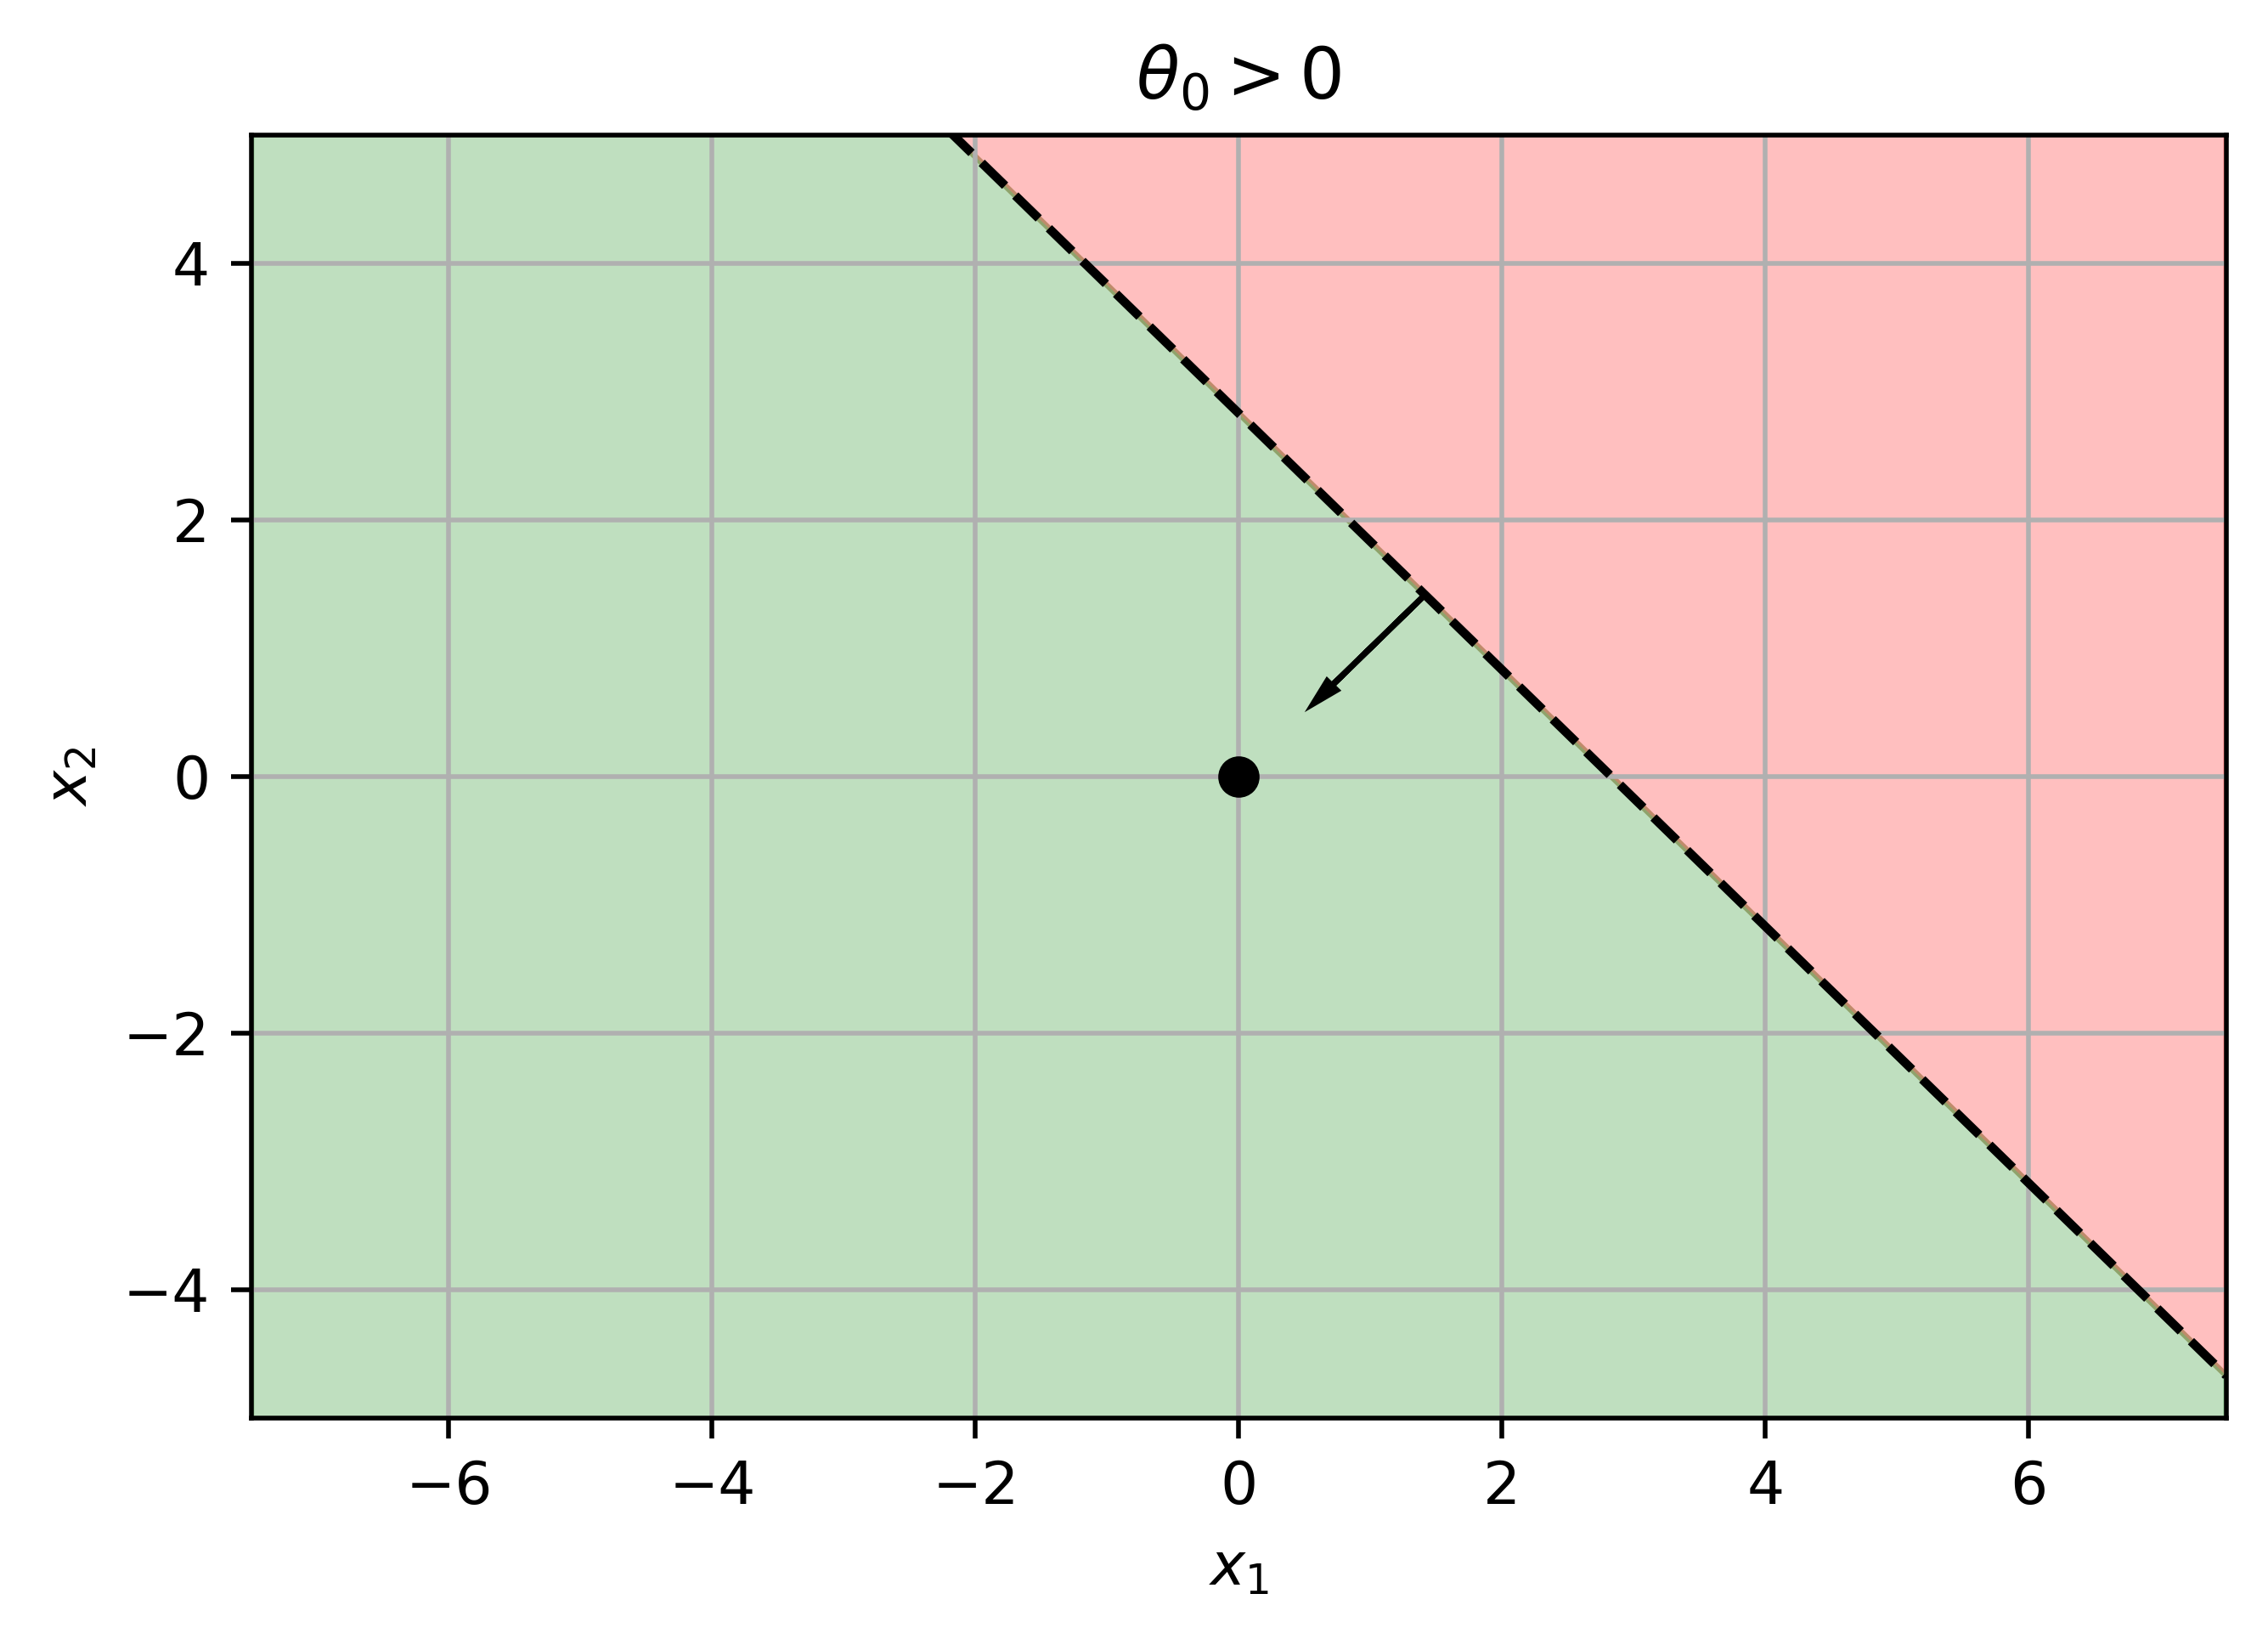
\includegraphics[width=60mm,scale=0.5]{images/classification_images/theta_0_greater_zero.png}
                    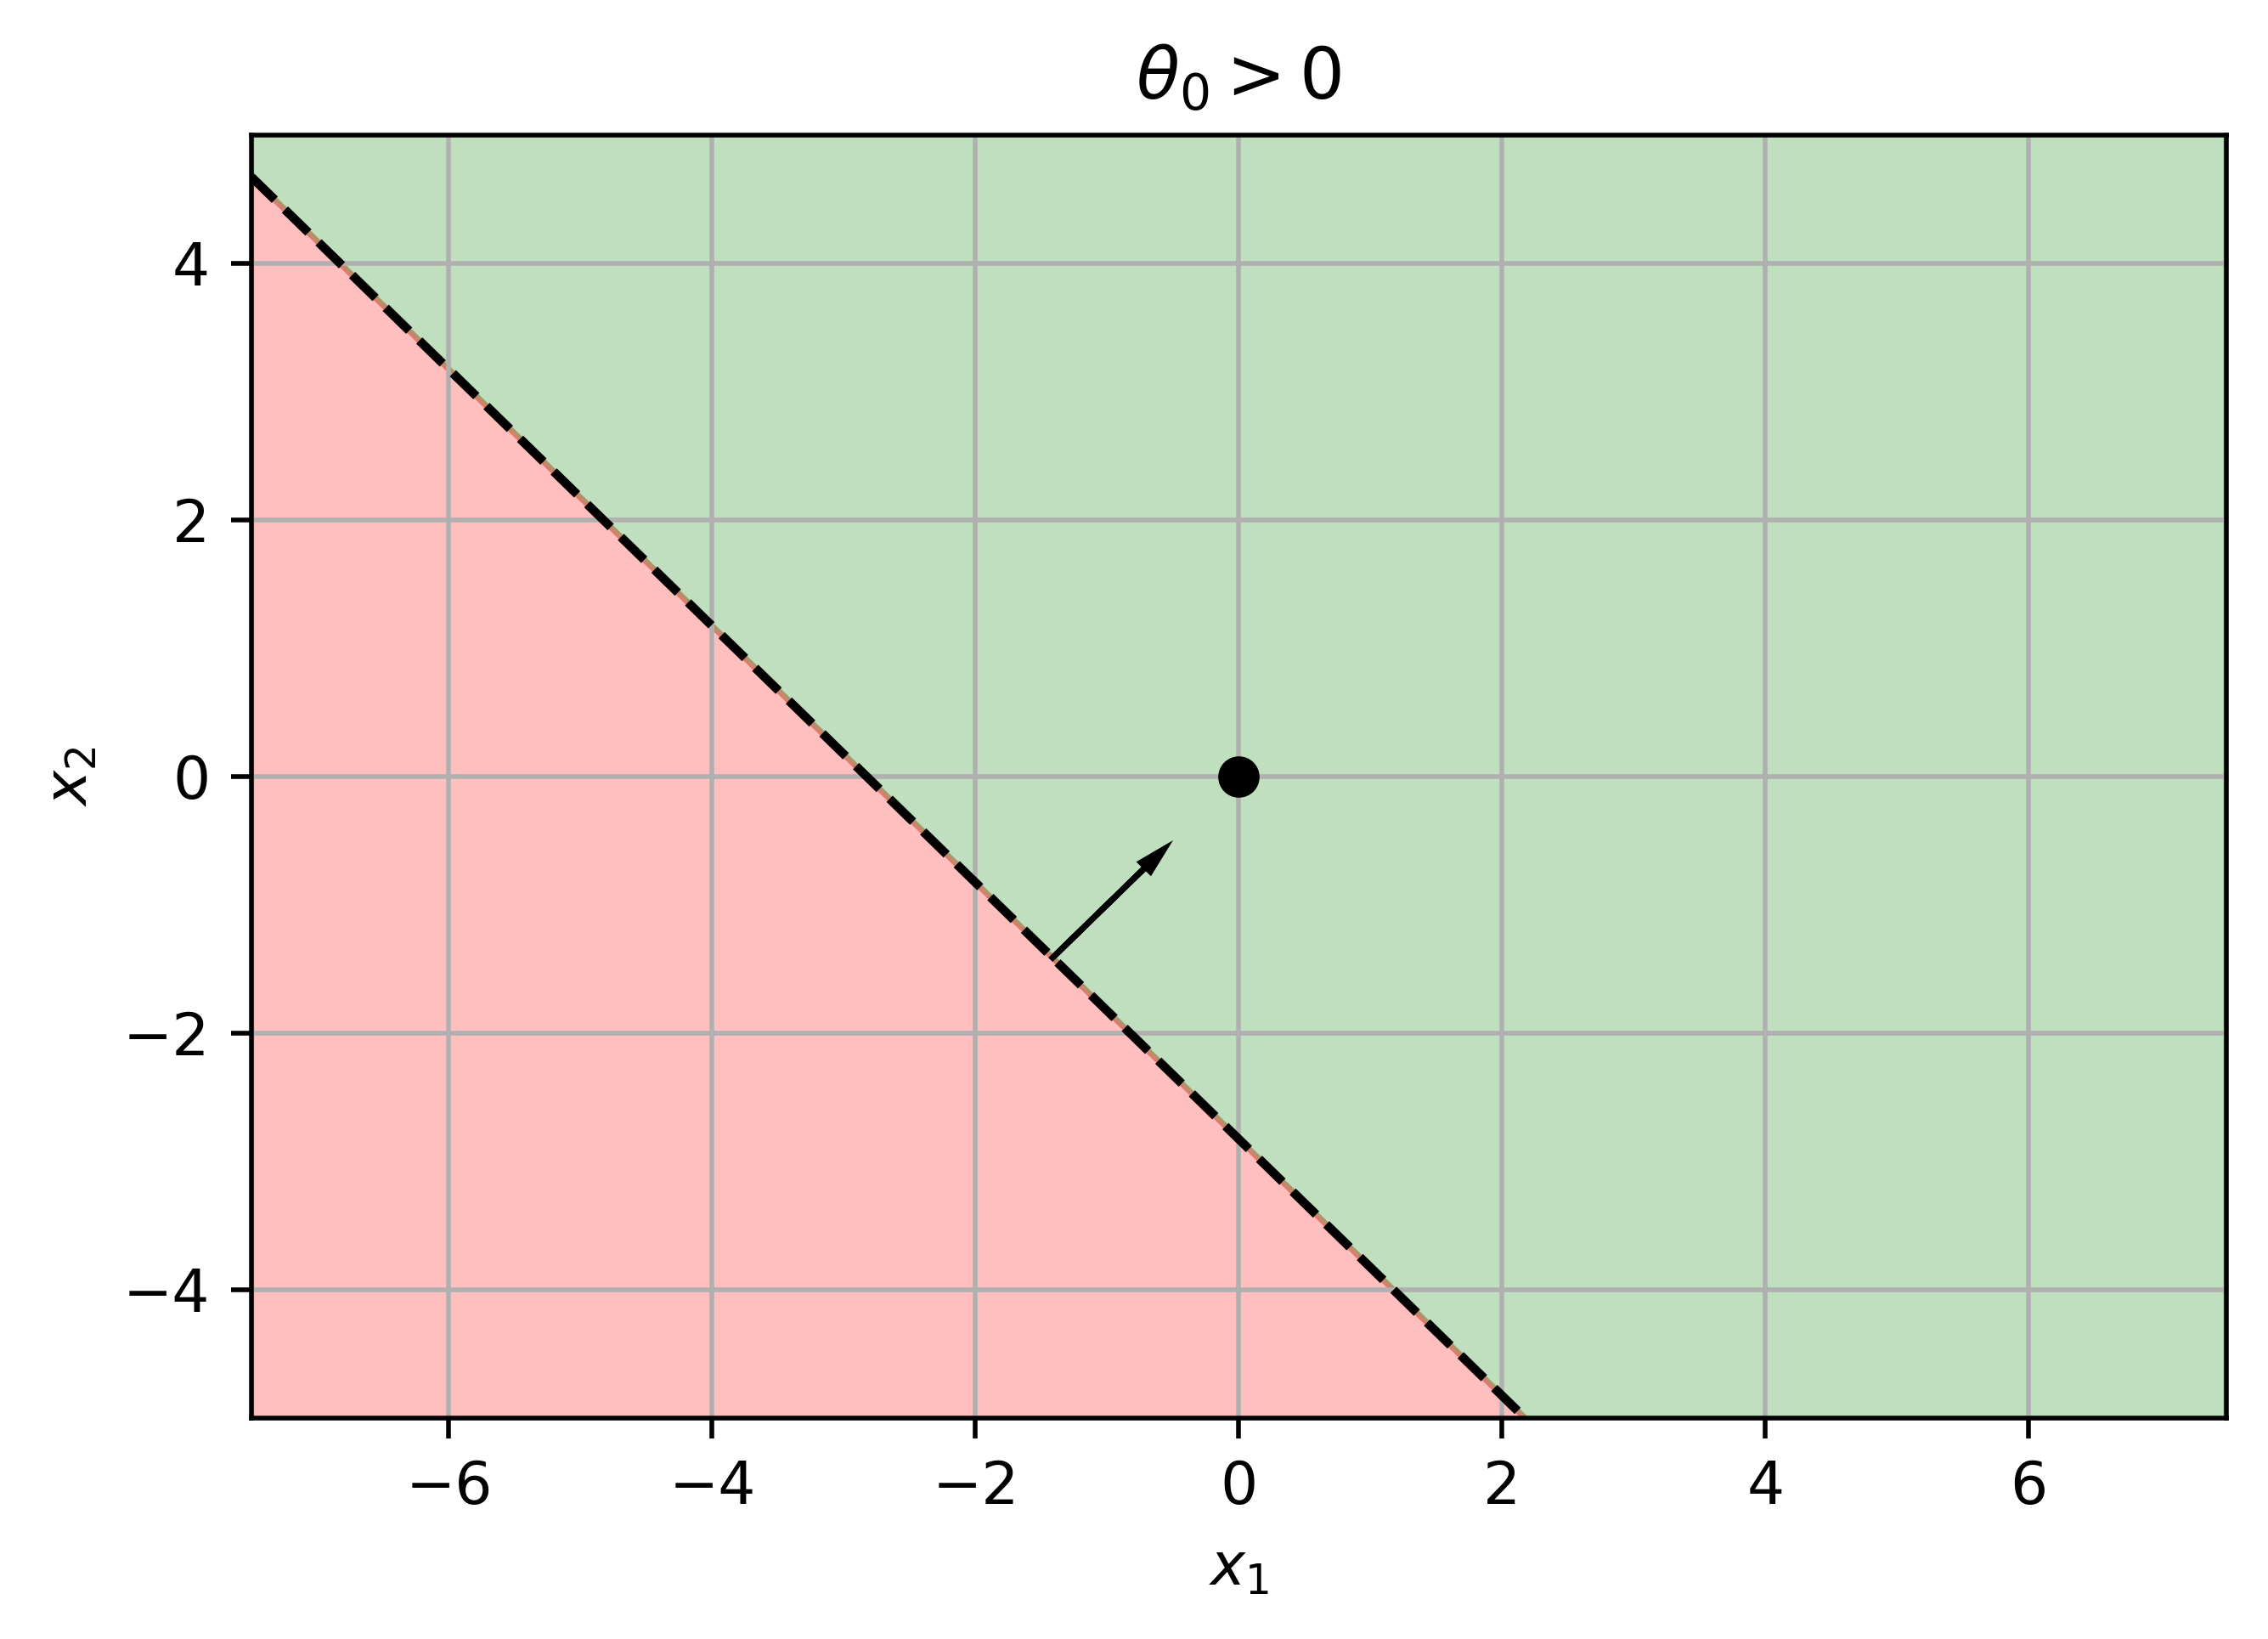
\includegraphics[width=60mm,scale=0.5]{images/classification_images/positive_theta0_positive_theta.png}
                        \caption*{If we have a \textbf{positive} constant, it's "easier" to get a positive \textbf{result}: more positive space.}
                \end{figure}
                
                
            \item If $\theta_0<0$, then $x=(0,0)$ is in the \textbf{negative} region.
                \begin{itemize}
                    \item That means the positive region is \textbf{smaller}: the line must have moved in the $+\theta$ direction.
                \end{itemize}
                
                \begin{figure}[H]
                    \centering                         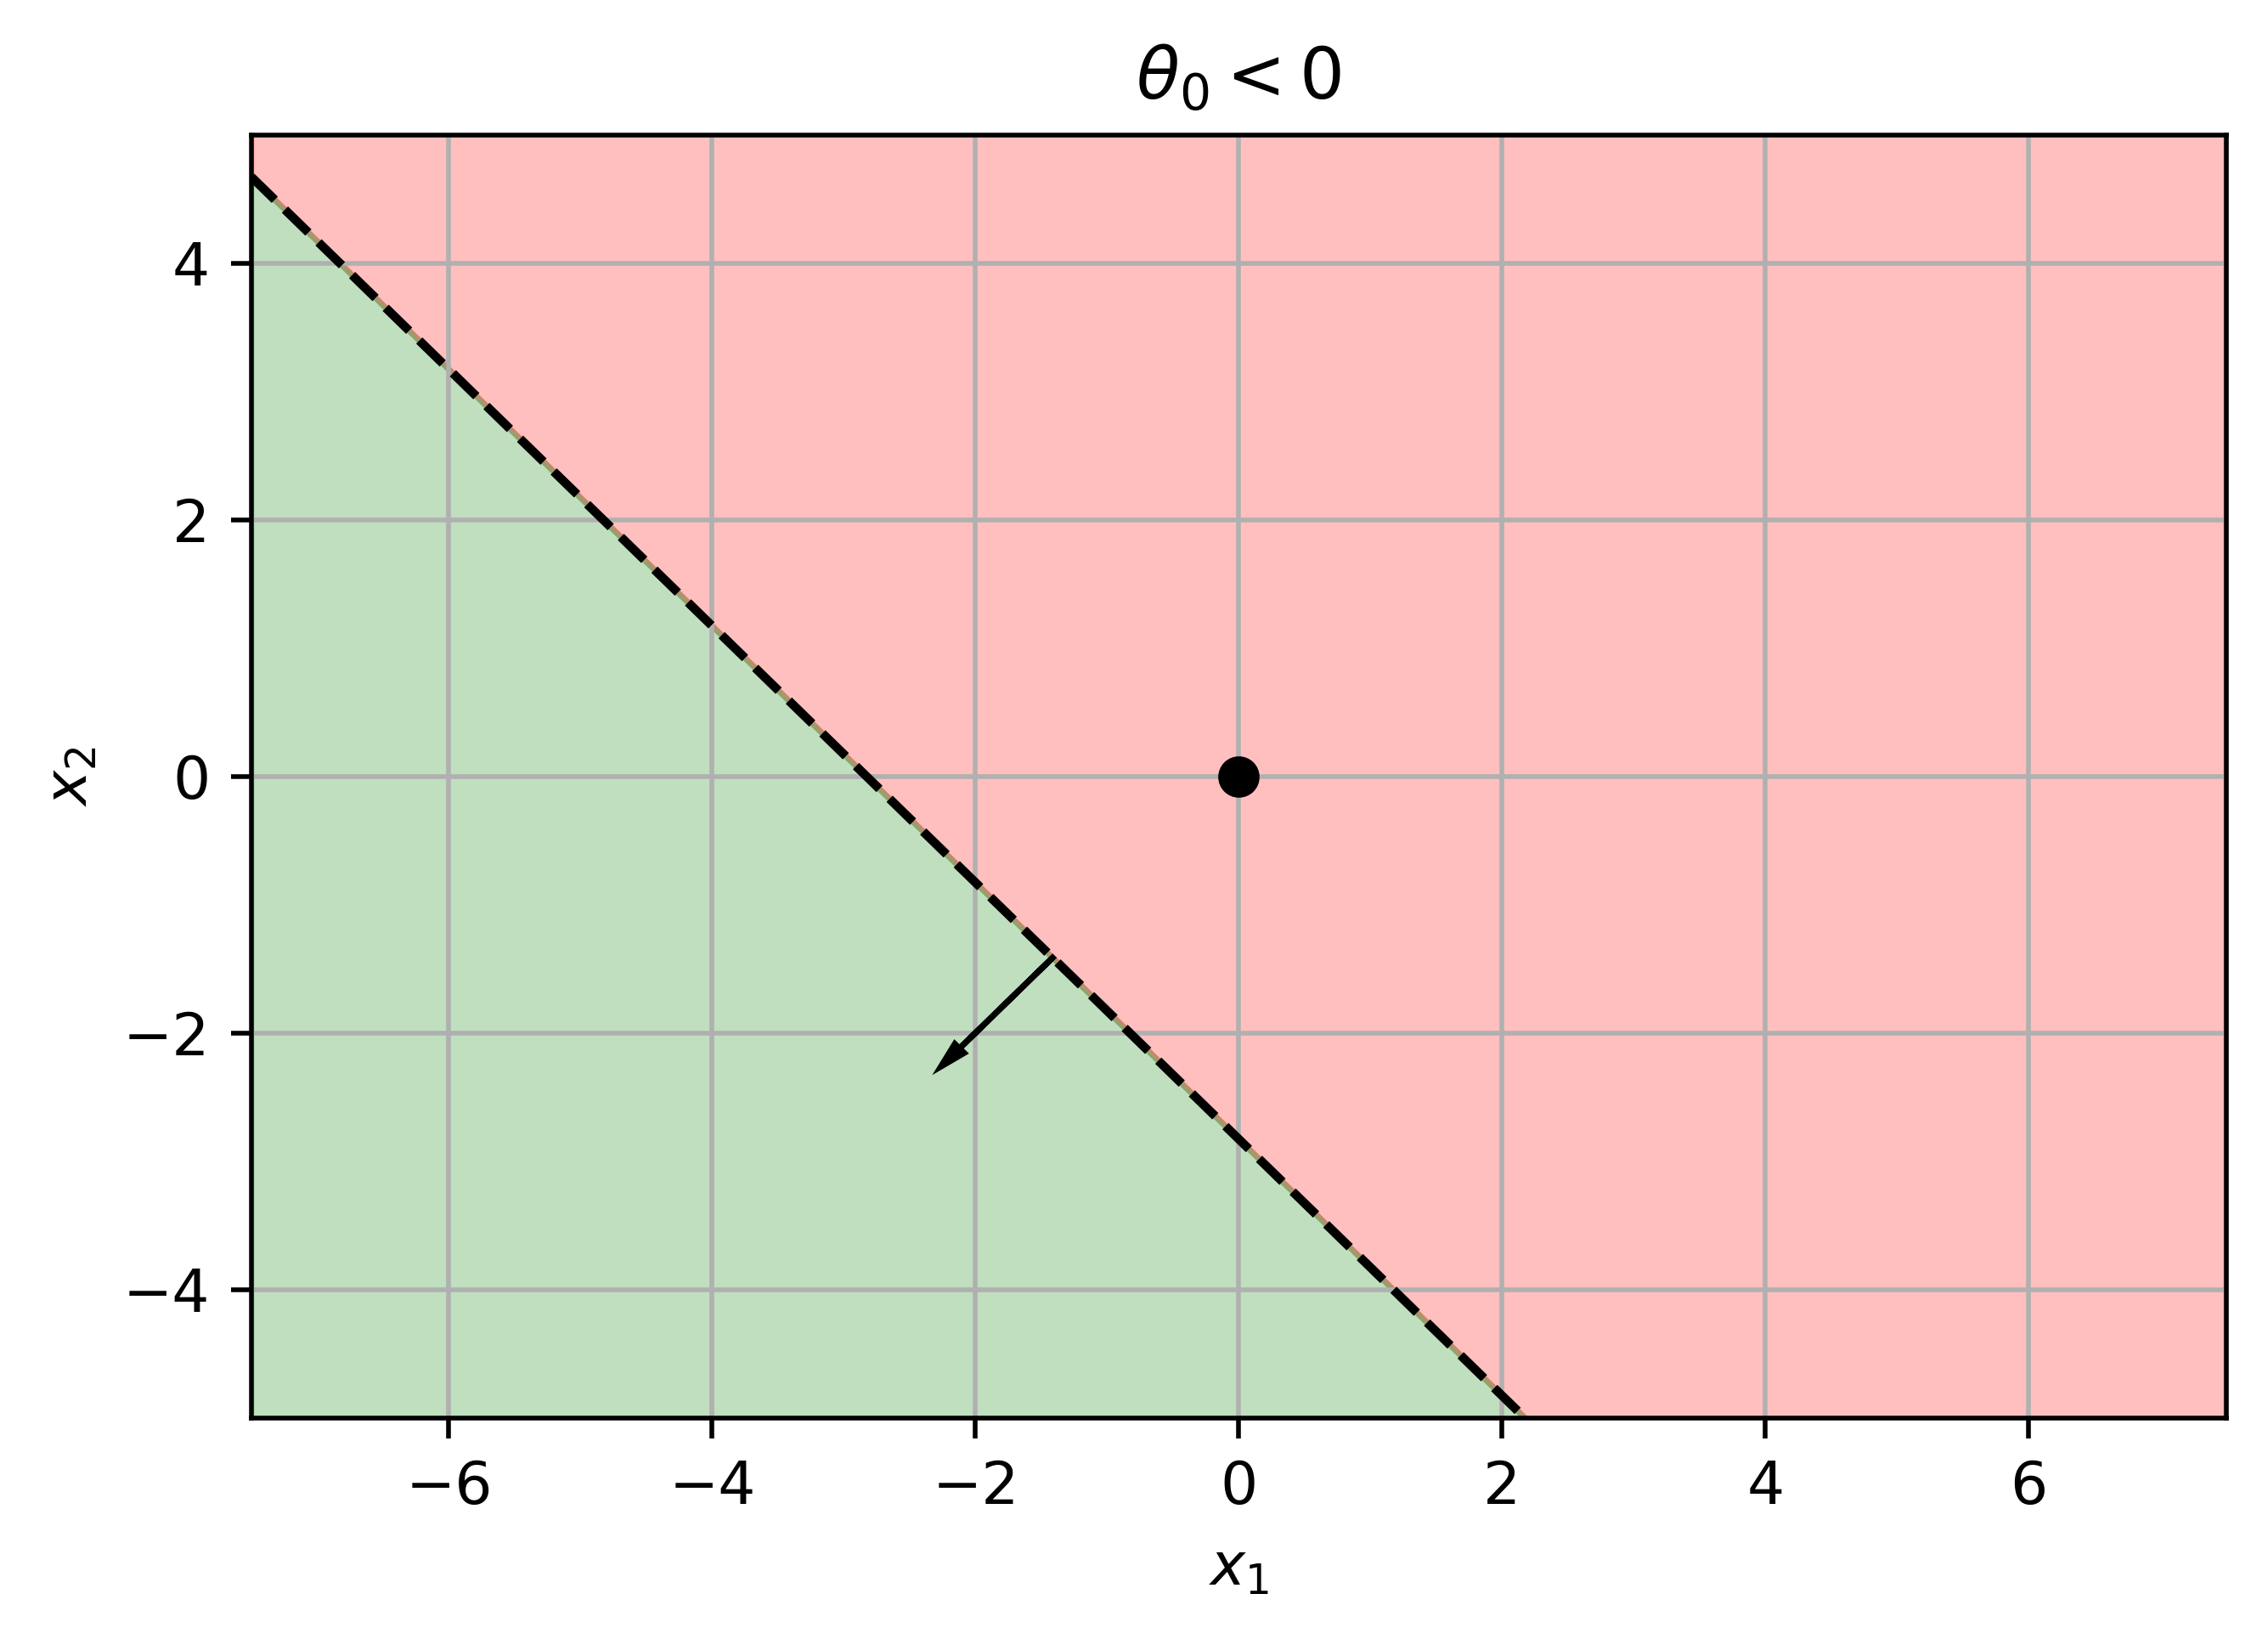
\includegraphics[width=60mm,scale=0.5]{images/classification_images/theta_0_less_zero.png}
                    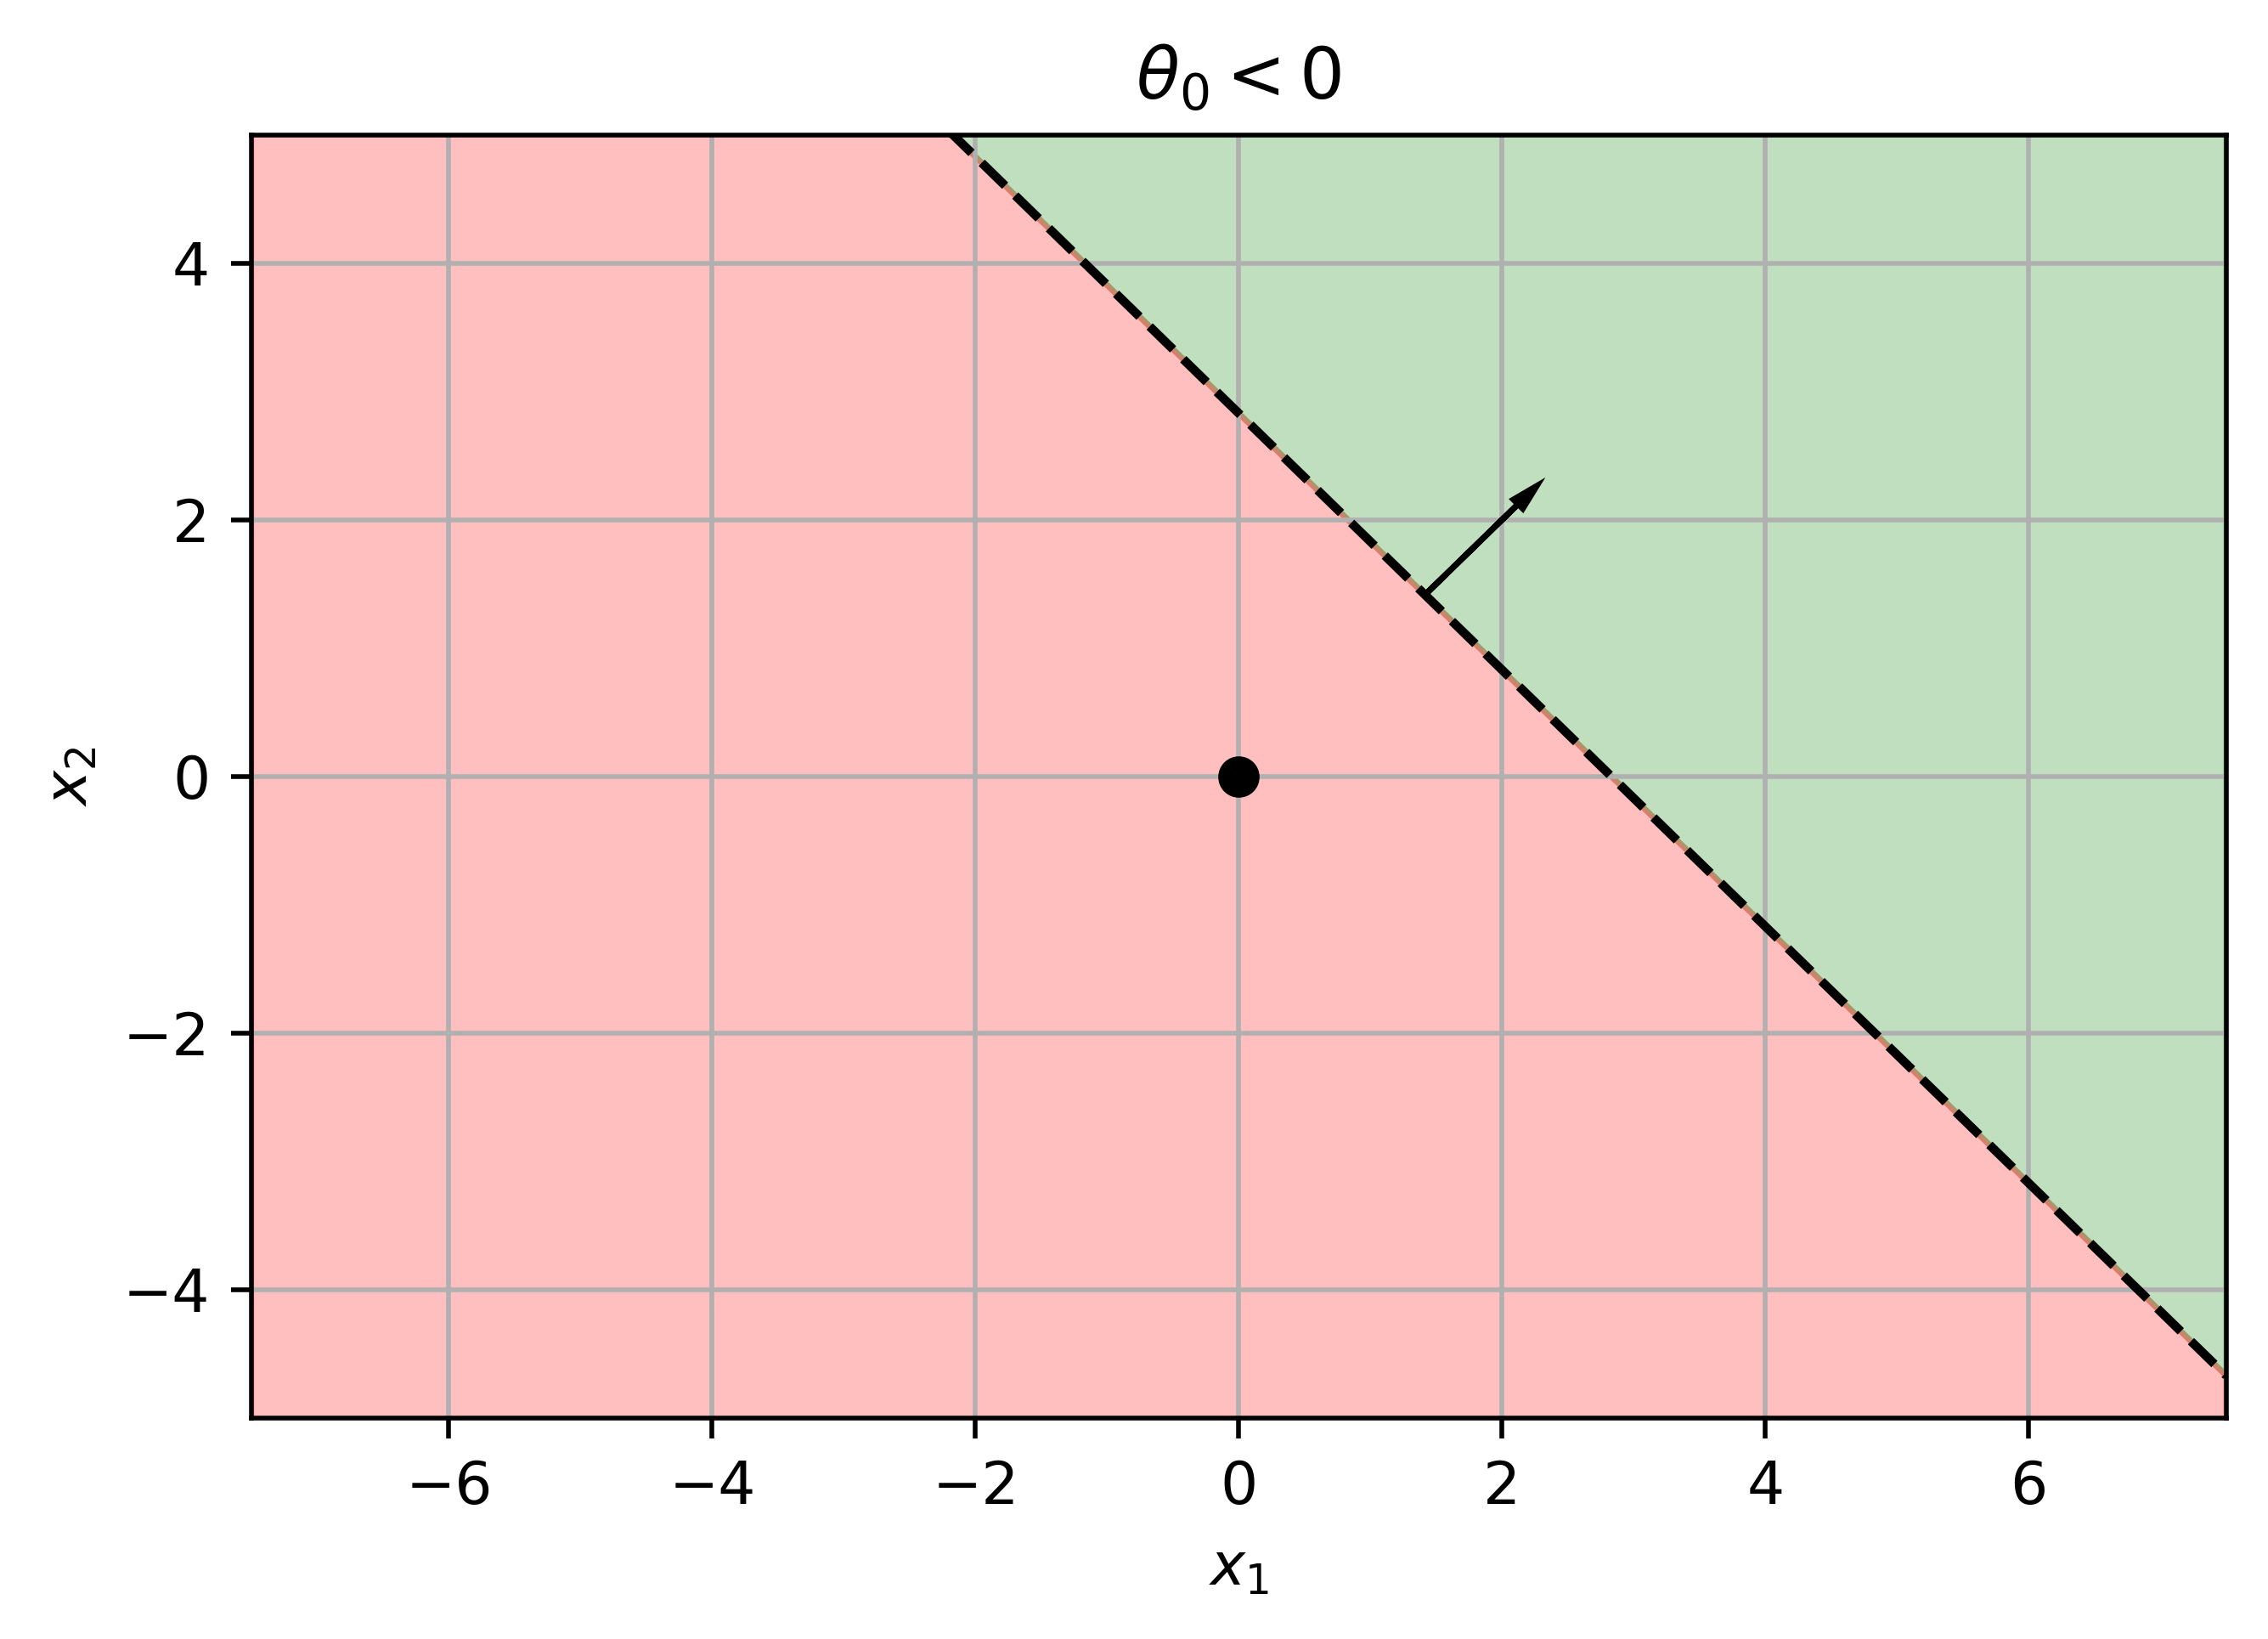
\includegraphics[width=60mm,scale=0.5]{images/classification_images/negative_theta0_positive_theta.png}
                        \caption*{If we have a \textbf{negative} constant, it's "harder" to get a positive \textbf{result}: more negative space.}
                \end{figure}
        \end{itemize}
        
        This can be a bit confusing, so we'll summarize:\\
        
            \begin{concept}
                The \gren{sign} of our $\theta_0$ and the \purp{direction} we move away from the origin are \vocab{opposite}.
                
                If \blu{$\theta_0>0$} (positive), our boundary moves in the \purp{$-\theta$ direction}.
                
                If \blu{$\theta_0<0$} (negative), our boundary moves in the \purp{$+\theta$ direction}.
            \end{concept}
        
        This gives us a general idea of how the offset affects it, but what is the \textbf{exact} effect of $\theta_0$ on the line?
        
        We'll focus on one point on the line: the \textbf{closest point to the origin} We want to look at this \textbf{point} because it's \textbf{unique}.
            \note{Points that aren't unique are hard to keep track of!}
    
    \subsection*{Distance from the Origin to the Plane}
    
        \begin{figure}[H]
            \centering
                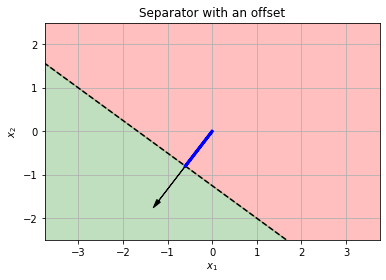
\includegraphics[width=70mm,scale=0.5]{images/classification_images/separator_with_offset_shown.png}
                \caption*{Notice that the \textbf{shortest} path from the origin to the line is \textbf{parallel} to $\theta$!}
        \end{figure}
        
        So, we can think of our \textbf{line} as having been \textbf{pushed} in the $\theta$ direction. This \textbf{matches} what we did for 1-D separators: $x_1>3$ was moved in the $x_1$ direction.
        
        So, we'll take the closest point on the line, $\vec{d}$. The \textbf{magnitude} $d$ will give us the \textbf{distance} that the separator has been \textbf{shifted}.
        
        \begin{figure}[H]
            \centering
                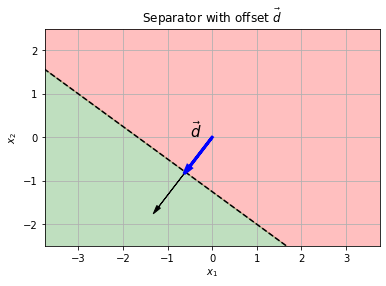
\includegraphics[width=70mm,scale=0.5]{images/classification_images/separator_with_offset_d.png}
        \end{figure}
        
        Since $\vec{d}$ is in the direction of $\theta$, the direction can be captured by the unit vector $\hat{\theta}$. Let's take a look at that:
            \note{Remember, a vector is direction (unit vector) times magnitude (scalar).}
            
        \begin{equation}
            \theta = \norm{\theta} \red{\hat{\theta}}
        \end{equation}
        
        \begin{equation}
            \vec{d} = d \red{\hat{\theta}}
        \end{equation}
        
        They're in the same \textbf{direction}, so they have the same \textbf{unit vector} $\hat{\theta}$.
        
        $\vec{d}$ is on the \textbf{line}, so it satisfies:
            \note{We'll use $\theta \cdot \vec{d}$ instead of $\theta^T \vec{d}$ here.}
        
        \begin{equation}
            \theta \cdot \vec{d} + \theta_0=0
        \end{equation}
        
        We can plug our equations 4.8 and 4.9, where we've separated magnitude from unit vector:
        
        \begin{equation}
        \overbrace{
            \Big(
                \norm{\theta} 
                \red{\hat{\theta}}
            \Big)
        }^{\theta}
        \cdot
        \overbrace{
            \Big(
            d \red{\hat{\theta}}
            \Big)
        }^{\vec{d}}
            + \theta_0
        \end{equation}
        
        We can move the scalars $\norm{\theta}$ and $d$ out of the way of the dot product:
        
        \begin{equation}
            \norm{\theta} d \left( 
                                \red{\hat{\theta} \cdot \hat{\theta}} 
                          \right) 
                          + \theta_0
        \end{equation}
        
        We know that $\hat{u} \cdot \hat{u}=1$:
        
        \begin{equation}
            \norm{\theta}d+\theta_0=0
        \end{equation}
        
        And now, we just solve for $d$:\\
        
        \begin{concept}
            The \vocab{distance} $d$ from the \purp{origin} to our \gren{linear separator} is 
            
            \begin{equation}
                d = \frac{ -\theta_0}{\norm{\theta}}
            \end{equation}
        \end{concept}
        
        A "negative" distance means $\vec{d}$ (the vector from the origin to the line) is pointed in the opposite direction of $\theta$.
        
        \begin{figure}[H]
            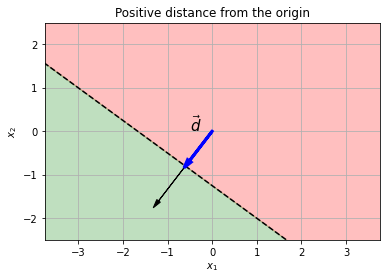
\includegraphics[width=70mm,scale=0.5]{images/classification_images/positive_distance.png}
            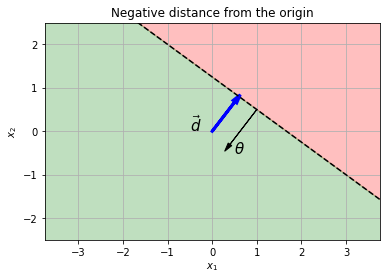
\includegraphics[width=70mm,scale=0.5]{images/classification_images/negative_distance.png}
            
        \end{figure}
        
        Notice, again, that this agrees with our \textbf{earlier} thought: the sign of $\theta_0$ is the opposite ($-1$) of the $\theta$ direction we move in.